\documentclass[11pt]{article}
\usepackage{amsmath,amssymb,amsthm}
\usepackage{geometry}
\usepackage{booktabs}
\usepackage{graphicx}
\usepackage{hyperref}
\usepackage{enumerate}
\usepackage{listings}
\usepackage{xcolor}
\usepackage{fancyhdr}
\usepackage{tikz}
\usetikzlibrary{arrows.meta,positioning,shapes.geometric,calc}

\geometry{letterpaper, margin=1in}

\lstset{
  basicstyle=\ttfamily\small,
  breaklines=true,
  columns=fullflexible,
  keepspaces=true,
  language=C++,
  keywordstyle=\color{blue}\bfseries,
  commentstyle=\color{gray},
  stringstyle=\color{red!60!black}
}

\pagestyle{fancy}
\fancyhf{}
\fancyhead[L]{\small Dev Day $\sim$42 --- Revised Notation}
\fancyhead[R]{\small VSEPR-SIM}
\fancyfoot[C]{\thepage}

\title{\textbf{Dev Day $\sim$42: Revised State Notation} \\
\Large State Machine with Physics-Informed Bookkeeping}
\author{VSEPR-SIM Development}
\date{Version 1.0.0 --- Revised Notation Draft}

\begin{document}
\maketitle
\tableofcontents
\newpage

% ====================================================================
\section{Motivation: Why the Old Notation Had to Go}
% ====================================================================

The symbol $I$ collides with literally every field in physics:
\begin{itemize}
  \item Electric current ($I = Q/t$)
  \item Moment of inertia ($I = mr^2$)
  \item Identity matrix ($I_n$)
  \item Intensity ($I = P/A$)
  \item Action integral ($I = \int L \, dt$)
  \item Ionization energy ($I_1, I_2, \ldots$)
  \item Nuclear spin quantum number
\end{itemize}

Using $I$ as the initial-state symbol guaranteed confusion in any document that also discusses electrostatics, rotational mechanics, matrix algebra, or spectroscopy.

The fix is simple: use a symbol that does not collide.

\begin{equation}
\boxed{S_0 = \{m_0, \; E_0, \; x_0, \; v_0, \; C, \; \mathcal{E}, \; K, \; \Sigma\}}
\end{equation}

$S_0$ is clean, neutral, and non-annoying.

% ====================================================================
\section{State Declaration (Initial Conditions)}
% ====================================================================

\subsection{Formal Definition}

The initial state container is:
\begin{equation}
S_0 = \{m_0, \; E_0, \; x_0, \; v_0, \; C, \; \mathcal{E}, \; K, \; \Sigma\}
\end{equation}

\begin{center}
\begin{tabular}{clp{8cm}}
\toprule
\textbf{Symbol} & \textbf{Name} & \textbf{Description} \\
\midrule
$S_0$ & Initial state container & Clean, neutral, non-annoying \\
$m_0$ & Initial mass & Total system mass (amu) \\
$E_0$ & Initial energy & Total system energy (kcal/mol) \\
$x_0$ & Spatial configuration & Center-of-mass position (\AA) \\
$v_0$ & Velocity / motion state & Center-of-mass velocity (\AA/ps) \\
$C$ & Composition & Atomistic / bead / hybrid / macro \\
$\mathcal{E}$ & Environment & $T$, $P$, fields, radiation, flow \\
$K$ & Constraints & Geometry, bonding rules, allowed transitions \\
$\Sigma$ & Source / provenance tags & Where did this state come from? \\
\bottomrule
\end{tabular}
\end{center}

\subsection{Design Rationale}

Each field has a clear physical or bookkeeping purpose:

\begin{itemize}
  \item \textbf{$m_0, E_0$}: Scalar aggregates. Even if the underlying state has $N$ particles with individual masses, the container-level mass and energy are always well-defined.
  \item \textbf{$x_0, v_0$}: The center-of-mass phase-space point. Individual particle coordinates live in the detailed \texttt{State} object that $S_0$ wraps.
  \item \textbf{$C$}: A bookkeeping tag, not a physics quantity. Tells the engine which force evaluators and integrators are valid.
  \item \textbf{$\mathcal{E}$}: External conditions that the system responds to but does not generate. Temperature, pressure, electric/magnetic fields, radiation flux, shear rate.
  \item \textbf{$K$}: Hard constraints that the engine must respect. Frozen atoms, bonding rules, symmetry groups.
  \item \textbf{$\Sigma$}: Provenance chain. If you cannot answer ``where did this number come from?'' then your simulation is not reproducible.
\end{itemize}

\subsection{What $S_0$ Does Not Contain}

$S_0$ intentionally omits:
\begin{itemize}
  \item Force vectors (these are computed, not stored)
  \item Scratch buffers (temporary workspace for integrators)
  \item Visualization state (rendering is a separate layer)
  \item File I/O handles (state is pure data)
\end{itemize}

% ====================================================================
\section{Outcome State}
% ====================================================================

\subsection{Formal Definition}

\begin{equation}
S_f = \{m_f, \; E_f, \; \Phi, \; \mathcal{S}, \; \Pi, \; \Omega, \; Q\}
\end{equation}

\begin{center}
\begin{tabular}{clp{8cm}}
\toprule
\textbf{Symbol} & \textbf{Name} & \textbf{Description} \\
\midrule
$S_f$ & Final state & The result of transformation \\
$m_f$ & Final mass & Total system mass after evolution \\
$E_f$ & Final energy & Total system energy after evolution \\
$\Phi$ & Structural state & Geometry/topology class \\
$\mathcal{S}$ & Stability metric & Thermodynamic and kinetic stability quantifier \\
$\Pi$ & Performance properties & Transport / material properties (diffusion, viscosity, etc.) \\
$\Omega$ & Event log & Reactions, transitions, failures during $T$ \\
$Q$ & Quality / confidence flags & How much should you trust this result? \\
\bottomrule
\end{tabular}
\end{center}

\subsection{Structural State ($\Phi$)}

$\Phi$ classifies the geometry and topology of the outcome:
\begin{itemize}
  \item Geometry class: linear, trigonal planar, tetrahedral, octahedral, \ldots
  \item Topology: chain, ring, branched, lattice, amorphous
  \item Symmetry score: 0 (no symmetry) to 1 (perfect)
  \item Coordination number (average)
\end{itemize}

\subsection{Event Log ($\Omega$)}

$\Omega$ records every discrete event during transformation:
\begin{itemize}
  \item Bond breaking / forming events
  \item Phase transitions
  \item Constraint violations (flagged, not silenced)
  \item Energy drift warnings
  \item Failure modes
\end{itemize}

Each event carries: step number, type tag, human-readable description, and associated energy change $\Delta E$.

\subsection{Quality Flags ($Q$)}

$Q$ is the honesty layer. It tells you:
\begin{itemize}
  \item Was energy conserved?
  \item Was mass conserved?
  \item Did forces converge?
  \item Were symmetry constraints respected?
  \item What is the absolute energy drift?
\end{itemize}

If $Q$ reports \texttt{energy\_conserved = false}, the result is suspect and the user is informed. The engine does NOT silently continue with broken bookkeeping.

% ====================================================================
\section{Transformation Layer}
% ====================================================================

\subsection{The Only Thing That Actually Matters}

\begin{equation}
\boxed{S_f = T(S_0, \; t, \; \Lambda)}
\end{equation}

\begin{center}
\begin{tabular}{clp{8cm}}
\toprule
\textbf{Symbol} & \textbf{Name} & \textbf{Description} \\
\midrule
$T$ & Transformation operator & Your engine \\
$t$ & Time / iteration domain & How long to run \\
$\Lambda$ & Model fidelity level & C-level here, not physics-resolved \\
\bottomrule
\end{tabular}
\end{center}

This is the whole point:

\begin{quote}
\textit{You are no longer solving reality. You are mapping states through controlled abstraction.}
\end{quote}

\subsection{Model Fidelity ($\Lambda$)}

The $\Lambda$ parameter tells the engine \textit{how much physics} to include:

\begin{center}
\begin{tabular}{clp{7cm}}
\toprule
\textbf{Level} & \textbf{Name} & \textbf{Description} \\
\midrule
$\Lambda_0$ & C-Empirical & Classical empirical: harmonic bonds, LJ, Coulomb \\
$\Lambda_1$ & C-Reactive & Classical with bond-order potentials (ReaxFF-like) \\
$\Lambda_2$ & C-Polarizable & Classical with induced dipoles / SCF polarization \\
$\Lambda_3$ & CG-Reduced & Coarse-grained reduced model \\
$\Lambda_4$ & CG-Enriched & Coarse-grained enriched descriptor model \\
$\Lambda_5$ & Hybrid-AdRes & Adaptive resolution (atomistic core + CG shell) \\
\bottomrule
\end{tabular}
\end{center}

At C-level ($\Lambda_0$ through $\Lambda_2$), we are not resolving quantum mechanics or electronic structure. We are mapping states through controlled classical approximation. The fidelity level is an explicit parameter, not a hidden assumption.

\subsection{Composability}

Because $T$ maps $S_0 \to S_f$, and $S_f$ can be wrapped back into an $S_0$ (with updated provenance), transformations compose:

\begin{equation}
S_f^{(3)} = T\bigl(T\bigl(T(S_0, \, t_1, \, \Lambda_a), \, t_2, \, \Lambda_b\bigr), \, t_3, \, \Lambda_c\bigr)
\end{equation}

This enables multi-fidelity workflows: optimize at $\Lambda_0$ (cheap), refine at $\Lambda_2$ (expensive), coarsen to $\Lambda_3$ (fast screening).

% ====================================================================
\section{Mass--Energy Sanity Constraint}
% ====================================================================

\subsection{Don't Let It Lie to You}

Even at C-level, enforce:

\begin{align}
E_0 + E_\text{in} - E_\text{out} &\approx E_f + E_\text{loss} \\
m_0 + m_\text{in} - m_\text{out} &\approx m_f
\end{align}

\begin{center}
\begin{tabular}{clp{7cm}}
\toprule
\textbf{Term} & \textbf{Name} & \textbf{Description} \\
\midrule
$E_0$ & Initial energy & From $S_0$ \\
$E_\text{in}$ & Injected energy & Thermostat, external fields, radiation \\
$E_\text{out}$ & Removed energy & Friction, thermostat coupling, damping \\
$E_f$ & Final energy & From $S_f$ \\
$E_\text{loss}$ & Dissipative loss & Explicitly tracked, never hidden \\
\midrule
$m_0$ & Initial mass & From $S_0$ \\
$m_\text{in}$ & Added mass & Particle creation events \\
$m_\text{out}$ & Removed mass & Particle destruction events \\
$m_f$ & Final mass & From $S_f$ \\
\bottomrule
\end{tabular}
\end{center}

If this drifts, your ``approximation layer'' quietly becomes fiction.

\subsection{Implementation}

The \texttt{EnergyBalance} struct tracks all six terms. At every step:

\begin{enumerate}
  \item Compute $\delta E = |(E_0 + E_\text{in} - E_\text{out}) - (E_f + E_\text{loss})|$
  \item If $\delta E > \varepsilon_E$: record a warning in $\Omega$, set $Q.\texttt{energy\_conserved} = \text{false}$
  \item Compute $\delta m = |(m_0 + m_\text{in} - m_\text{out}) - m_f|$
  \item If $\delta m > \varepsilon_m$: same treatment
\end{enumerate}

The tolerances $\varepsilon_E$ and $\varepsilon_m$ are explicit parameters in \texttt{TransformConfig}. They are not hidden. They are not ``close enough.'' They are the contract between the engine and the user.

% ====================================================================
\section{What You Actually Built}
% ====================================================================

Whether you admit it or not, this system is:

\begin{enumerate}
  \item \textbf{A state machine} --- $S_0 \to S_f$ with well-defined transitions
  \item \textbf{With physics-informed bookkeeping} --- mass-energy balance, provenance, quality flags
  \item \textbf{Feeding a multi-scale transformation engine} --- $\Lambda$ selects fidelity from atomistic through coarse-grained to hybrid
  \item \textbf{With traceable data lineage} --- $\Sigma$ provenance tags chain through every transformation
\end{enumerate}

Which is exactly what serious simulation frameworks do, except they pretend it is more mystical.

\subsection{State Machine Diagram}

\begin{center}
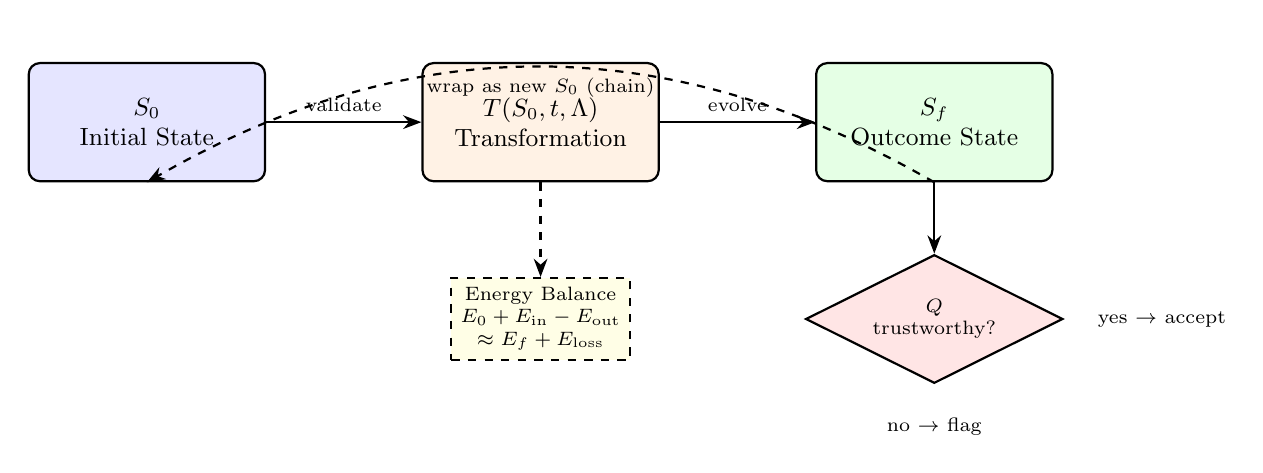
\begin{tikzpicture}[
  state/.style={rectangle, draw, rounded corners, minimum width=3cm,
    minimum height=1.5cm, font=\small, align=center},
  ->,>=Stealth, thick
]
  \node[state, fill=blue!10] (s0) at (0,0)
    {$S_0$\\Initial State};
  \node[state, fill=orange!10] (T) at (5,0)
    {$T(S_0, t, \Lambda)$\\Transformation};
  \node[state, fill=green!10] (sf) at (10,0)
    {$S_f$\\Outcome State};

  \draw (s0) -- node[above, font=\scriptsize] {validate} (T);
  \draw (T) -- node[above, font=\scriptsize] {evolve} (sf);

  % Feedback loop (composability)
  \draw[dashed, bend right=30] (sf.south) to
    node[below, font=\scriptsize] {wrap as new $S_0$ (chain)} (s0.south);

  % Quality gate
  \node[diamond, draw, fill=red!10, aspect=2, font=\scriptsize, align=center]
    (q) at (10, -2.5) {$Q$\\trustworthy?};
  \draw (sf) -- (q);
  \node[font=\scriptsize, right=0.3cm of q] {yes $\to$ accept};
  \node[font=\scriptsize, below=0.3cm of q] {no $\to$ flag};

  % Energy balance
  \node[rectangle, draw, dashed, fill=yellow!10, font=\scriptsize, align=center]
    (eb) at (5, -2.5) {Energy Balance\\$E_0 + E_\text{in} - E_\text{out}$\\$\approx E_f + E_\text{loss}$};
  \draw[dashed] (T) -- (eb);
\end{tikzpicture}
\end{center}

% ====================================================================
\section{C++ Implementation}
% ====================================================================

\subsection{StateC: The Initial State Container}

\begin{lstlisting}[caption={StateC --- Dev Day $\sim$42 initial state (atomistic/core/state\_c.hpp)}]
struct StateC {
    double mass;           // m_0
    double energy;         // E_0
    Vec3   position;       // x_0
    Vec3   velocity;       // v_0

    Composition   comp;         // C
    Environment   env;          // E (calligraphic)
    Constraints   constraints;  // K
    SourceTag     provenance;   // Sigma
};
\end{lstlisting}

\subsection{The Transformation Operator}

\begin{lstlisting}[caption={evolve --- The engine becomes a function}]
StateC evolve(const StateC& s0, double dt, ModelLevel level);
\end{lstlisting}

And the full-output version:

\begin{lstlisting}[caption={Full evolve with OutcomeState}]
OutcomeState evolve(const StateC& s0, const TransformConfig& config);
\end{lstlisting}

\subsection{Composition Enum}

\begin{lstlisting}
enum class Composition : uint8_t {
    Atomistic = 0,   // Full atomic resolution
    Bead      = 1,   // Coarse-grained bead
    Hybrid    = 2,   // Mixed atomistic + bead
    Macro     = 3    // Continuum / macro-scale
};
\end{lstlisting}

\subsection{ModelLevel Enum ($\Lambda$)}

\begin{lstlisting}
enum class ModelLevel : uint8_t {
    C_Empirical   = 0,  // Harmonic bonds, LJ, Coulomb
    C_Reactive    = 1,  // Bond-order potentials
    C_Polarizable = 2,  // Induced dipoles / SCF
    CG_Reduced    = 3,  // Coarse-grained reduced
    CG_Enriched   = 4,  // CG enriched descriptor
    Hybrid_AdRes  = 5   // Adaptive resolution
};
\end{lstlisting}

\subsection{EnergyBalance: The Honesty Ledger}

\begin{lstlisting}[caption={EnergyBalance --- mass-energy sanity constraint}]
struct EnergyBalance {
    double E_0{}, E_in{}, E_out{}, E_f{}, E_loss{};
    double m_0{}, m_in{}, m_out{}, m_f{};

    double energy_drift() const {
        return std::abs((E_0 + E_in - E_out) - (E_f + E_loss));
    }
    double mass_drift() const {
        return std::abs((m_0 + m_in - m_out) - m_f);
    }
    bool energy_sane(double tol = 1e-6) const {
        return energy_drift() < tol;
    }
    bool mass_sane(double tol = 1e-10) const {
        return mass_drift() < tol;
    }
};
\end{lstlisting}

% ====================================================================
\section{Integration with Existing Codebase}
% ====================================================================

\subsection{Relationship to atomistic::State}

The existing \texttt{atomistic::State} struct (defined in \texttt{atomistic/core/state.hpp}) is the detailed particle-level state:

\begin{equation}
\texttt{State} = (N, \, X, \, V, \, T, \, Q, \, M, \, \texttt{type}, \, B, \, L, \, F, \, E, \, \texttt{box})
\end{equation}

\texttt{StateC} wraps this with:
\begin{itemize}
  \item Container-level aggregates ($m_0$, $E_0$, $x_0$, $v_0$)
  \item Bookkeeping metadata ($C$, $\mathcal{E}$, $K$, $\Sigma$)
  \item A \texttt{const State*} pointer for zero-copy access to the detailed data
\end{itemize}

The factory method:
\begin{lstlisting}
StateC sc = StateC::from_state(full_state, provenance_tag);
\end{lstlisting}

computes the COM position/velocity and total mass/energy from the full particle data.

\subsection{Relationship to SimulationState}

The existing \texttt{vsepr::SimulationState} (in \texttt{src/sim/sim\_state.hpp}) is the engine-side state machine that owns the molecule, coordinates, velocities, forces, and integrator state. It corresponds to the \textit{interior} of the transformation operator $T$.

In the revised notation:
\begin{itemize}
  \item \texttt{StateC} = the \textit{contract} at the boundary (what goes in, what comes out)
  \item \texttt{SimulationState} = the \textit{mechanism} inside $T$ (how integration happens)
\end{itemize}

\subsection{Relationship to CGSystemState}

The existing \texttt{vsepr::cli::CGSystemState} (in \texttt{include/cli/system\_state.hpp}) holds beads, environment states, and scene metadata. In the revised notation, this is a specialized $S_0$ with $C = \text{Bead}$.

The \texttt{Composition} enum makes this explicit: when $C = \text{Bead}$, the engine knows to use coarse-grained force evaluators and CG integrators.

% ====================================================================
\section{Multi-Fidelity Workflow Example}
% ====================================================================

\begin{enumerate}
  \item \textbf{Parse input}: Load \texttt{water\_cluster.xyz} into \texttt{atomistic::State}
  \item \textbf{Wrap}: \texttt{StateC s0 = StateC::from\_state(state, \{.origin="file:water\_cluster.xyz"\})}
  \item \textbf{Optimize} (cheap): \texttt{auto s1 = evolve(s0, 0.1, ModelLevel::C\_Empirical)}
  \item \textbf{Refine} (expensive): \texttt{auto s2 = evolve(s1, 0.001, ModelLevel::C\_Polarizable)}
  \item \textbf{Coarsen}: Map atomistic result to beads, set $C = \text{Bead}$
  \item \textbf{Screen} (fast): \texttt{auto s3 = evolve(s2\_cg, 1.0, ModelLevel::CG\_Reduced)}
  \item \textbf{Inspect}: Check $Q$ flags at each stage. If any report \texttt{energy\_conserved = false}, the pipeline stops.
\end{enumerate}

Each step carries its provenance in $\Sigma$. The chain is:
\begin{equation}
\Sigma: \; \texttt{file:water\_cluster.xyz} \to \texttt{evolve}(\Lambda_0) \to \texttt{evolve}(\Lambda_2) \to \texttt{coarsen} \to \texttt{evolve}(\Lambda_3)
\end{equation}

% ====================================================================
\section{Relationship to Deep Research Engine}
% ====================================================================

The Deep Research Engine (\texttt{atomistic/research/deep\_research.hpp}) implements a 4-phase pipeline:

\begin{center}
\begin{tabular}{clcl}
\toprule
\textbf{Phase} & \textbf{Name} & \textbf{$C$} & \textbf{$\Lambda$} \\
\midrule
10A & Atomistic Enumeration & Atomistic & $\Lambda_0$ (C-Empirical) \\
20B & Bead Formation & Bead & $\Lambda_3$ (CG-Reduced) \\
31C & MD Assembly & Bead & $\Lambda_3$ (CG-Reduced) \\
41A & Lattice Assembly & Macro & --- (blank call) \\
\bottomrule
\end{tabular}
\end{center}

In the revised notation, each phase is a transformation:
\begin{align}
S_f^{(10A)} &= T(S_0^{\text{seed}}, \; t_{10A}, \; \Lambda_0) \\
S_f^{(20B)} &= T(S_f^{(10A)} \to \text{Bead}, \; t_{20B}, \; \Lambda_3) \\
S_f^{(31C)} &= T(S_f^{(20B)}, \; t_{31C}, \; \Lambda_3) \\
S_f^{(41A)} &= T(S_f^{(31C)} \to \text{Macro}, \; 0, \; \text{infer})
\end{align}

The SHA-512 hash system in the deep research engine maps directly to the $\Sigma$ provenance tags: each pathway fingerprint becomes a \texttt{SourceTag.hash}.

% ====================================================================
\section{Project Tree Context}
% ====================================================================

\begin{lstlisting}[basicstyle=\ttfamily\scriptsize]
atomistic/
  core/
    state.hpp           <-- Particle-level state (N, X, V, M, ...)
    state_c.hpp         <-- Dev Day ~42 revised notation (THIS FILE)
    linalg.hpp
  integrators/
    fire.hpp            <-- FIRE optimizer (used inside T)
  research/
    deep_research.hpp   <-- 4-phase pipeline (uses StateC notation)
  reaction/
    discovery.hpp       <-- Discovery engine (reaction mining)

coarse_grain/
  core/
    bead.hpp            <-- Bead struct (C = Bead representation)
    environment_state.hpp <-- Environment-responsive state (X_B)
  models/
    model_selector.hpp  <-- ModelTier (maps to Lambda levels)

src/sim/
  sim_state.hpp         <-- SimulationState (interior of T)
  optimizer.hpp         <-- FIRE parameters

include/cli/
  system_state.hpp      <-- CGSystemState (C = Bead specialization)

docs/
  section2_state_ontology.tex          <-- Original state ontology
  section_state_c_revised_notation.tex <-- THIS DOCUMENT
\end{lstlisting}

% ====================================================================
\section{Symbol Reference}
% ====================================================================

Complete symbol table for the revised notation:

\begin{center}
\begin{tabular}{cllp{6cm}}
\toprule
\textbf{Symbol} & \textbf{LaTeX} & \textbf{C++ Type} & \textbf{Meaning} \\
\midrule
$S_0$ & \verb|S_0| & \texttt{StateC} & Initial state container \\
$S_f$ & \verb|S_f| & \texttt{OutcomeState} & Outcome state \\
$T$ & \verb|T| & \texttt{evolve()} & Transformation operator \\
$t$ & \verb|t| & \texttt{TransformConfig} & Time / iteration domain \\
$\Lambda$ & \verb|\Lambda| & \texttt{ModelLevel} & Model fidelity level \\
\midrule
$m_0$ & \verb|m_0| & \texttt{double mass} & Initial total mass \\
$E_0$ & \verb|E_0| & \texttt{double energy} & Initial total energy \\
$x_0$ & \verb|x_0| & \texttt{Vec3 position} & COM position \\
$v_0$ & \verb|v_0| & \texttt{Vec3 velocity} & COM velocity \\
$C$ & \verb|C| & \texttt{Composition} & Representation level \\
$\mathcal{E}$ & \verb|\mathcal{E}| & \texttt{Environment} & External conditions \\
$K$ & \verb|K| & \texttt{Constraints} & Rules / restrictions \\
$\Sigma$ & \verb|\Sigma| & \texttt{SourceTag} & Provenance tags \\
\midrule
$\Phi$ & \verb|\Phi| & \texttt{StructuralState} & Geometry/topology class \\
$\mathcal{S}$ & \verb|\mathcal{S}| & \texttt{StabilityMetric} & Stability quantifier \\
$\Pi$ & \verb|\Pi| & \texttt{PerformanceProperties} & Transport properties \\
$\Omega$ & \verb|\Omega| & \texttt{EventLog} & Event log \\
$Q$ & \verb|Q| & \texttt{QualityFlags} & Confidence flags \\
\bottomrule
\end{tabular}
\end{center}

% ====================================================================
\section{Summary}
% ====================================================================

Dev Day $\sim$42 establishes the revised notation for the VSEPR-SIM state machine:

\begin{enumerate}
  \item \textbf{$S_0$ replaces $I$} as the initial state symbol. No more collisions with current, inertia, identity, or intensity.
  \item \textbf{$S_f = T(S_0, t, \Lambda)$} is the only equation that matters. Everything else is bookkeeping to make $T$ honest.
  \item \textbf{Mass-energy sanity} is enforced at every step, not assumed. If it drifts, $Q$ flags it.
  \item \textbf{Provenance ($\Sigma$)} chains through every transformation, making the entire pipeline reproducible and inspectable.
  \item \textbf{Composition ($C$)} and \textbf{fidelity ($\Lambda$)} are explicit parameters, not hidden assumptions.
\end{enumerate}

The C++ implementation lives in \texttt{atomistic/core/state\_c.hpp} and integrates with the existing \texttt{atomistic::State}, \texttt{SimulationState}, and \texttt{CGSystemState} without breaking any existing interfaces.

\end{document}
